\chapter{LOCAL MOTOR INVARIANT}
\label{chap:li}

\nomenclature[f1]{$G$}{A Lie Group}
\nomenclature[f2]{$g_a$}{an element in Lie Group $G$ with parameter $a$}
\nomenclature[f3]{$I(x)$}{Invariant Function of $x$}
\nomenclature[f4]{$\ep$}{The parameter of a lie group element}
\graphicspath{{LocalInvariant/LocalInvariantFigs/EPS/}{LocalInvariant/LocalInvariantFigs/}}
It is not enough that animals are able to maintain the global motor invariant.
For a fish, preserving \emph{Global Motor Invariant}  means the swimming is stable and can be sustained.
However,  a fish also needs to adjust the speed and direction during swimming, which is of crucial importance for survival.
In real-life, animal can adapt motion primitives according to its purpose precisely.
In this chapter, we will develop the control strategies for tweaking motion patterns according to the motion purposes.

It is important to remember that such tweaking strategies are also constrained by the computation and memory capacity of the neural system, and should explore natural dynamics as the basic motion primitive theory. 
For \cms, it is of no meaning developing walking pattern by exploring natural dynamics but using optimization to adjust the walking speed. 
To meet such requirements, \moit\ adopted different ideas.

At first, when tweaking motion patterns, stability should not be violated. 
As stated in the previous chapter, a topological conjugation (one-one continuous invertible mapping)maintains the topology thus maintains the qualitative stability. Thus the ``tweaking'' action should be a topology conjugation. In an alternative perspective, such operations form a group and permit a combination operation. 

According to Group Theory, this means if two tweaking actions preserve the stability separately, the combination of the two actions also preserve the stability.
The space of topology conjugation is very large.
Currently, \moit\ only investigates a subset called \emph{The Lie Transformation Group} that is supported by the biological research studies and can be calculated efficiently.
The selected groups can be divided into orthodox subgroups, each of which is continuous and can be parameterized by one parameter.
In \cms, such parameters are closely related to motion purposes such as walking speed or swimming direction.

From the dynamic perspective, ``tweaking''  should also explore natural dynamics (passive based) as primitives.
Methods adopted in \moit\ belong to  a popular passive-based control principle, which carries many names: Controlled Symmetry, Controlled Lagrange, or Potential Shaping.
Different names reflect the fact that this method can be developed through different ways.
Roughly speaking, the original dynamic system is transformed according to motion purpose, the kinematics is untouched and control is applied by modifying the potential energy.
Such methods suit biological actuators like muscles and are also computationally efficient:
Closed form formula are developed for converting tweaking parameters to control effort.

This chapter is laid out in this way:
Section~\ref{sec:groupandsymmetry} introduces the basic idea of group and symmetry from intuitive geometry examples to more abstract algebraic formulation. Section~\ref{sec:liecontrol} investigates application of the Controlled Lagrange Method.
At last an example is provided in Section~\ref{sec:symball} to illustrate the idea.

In theory the ideas of group and invariant are closely related, like the two sides of a coin.
Group are the transformations which keep certain property invariant.
When searching for the group transformation, the invariant property is also determined.

In Motor Invariant Theory, the quantitative properties that are  preserved during group transformation are called \emph{Local Motor Invariant}.







\section{Group and Symmetry}
\label{sec:groupandsymmetry}
%To make motions realistic, some natural looking features should also be preserved.
%Some features of motions such as smoothness or energy efficient are quantitative.
%\cms research should provide a framework preserving feature.
%Another question mission is animals can finish motion tasks require high accuracy.
%
%These are the motivations for the development of \emph{Local Motor Invariant}.
%Local Motor Invariants are quantitative properties of motions, the idea of invariant preserving are abstracted as the ``Symmetry'' and Group theory.
%Features are modelled as symmetrical functions, while feature preserving actions form a group.
%From dynamic perspective, motions are solutions to dynamic equations.
%The actions transform one motion to another close related to the Lie Group Theory for differential equations\citep{olver1986applications}.
%
%The introduction of Lie Group not only provides a powerful mathematical tools for modelling the symmetry property, but also provides an idea to simplify the solving the dynamics.



For the more traditional geometrical perspective, ``Symmetry''  means a geometry is the same after certain transformation.
For example, a square remains the same shape after  $90$ degree clockwise rotation, as shown in Figure~\ref{fig:symsquare}.
\begin{figure}[!htbp]
  	\begin{center}
   	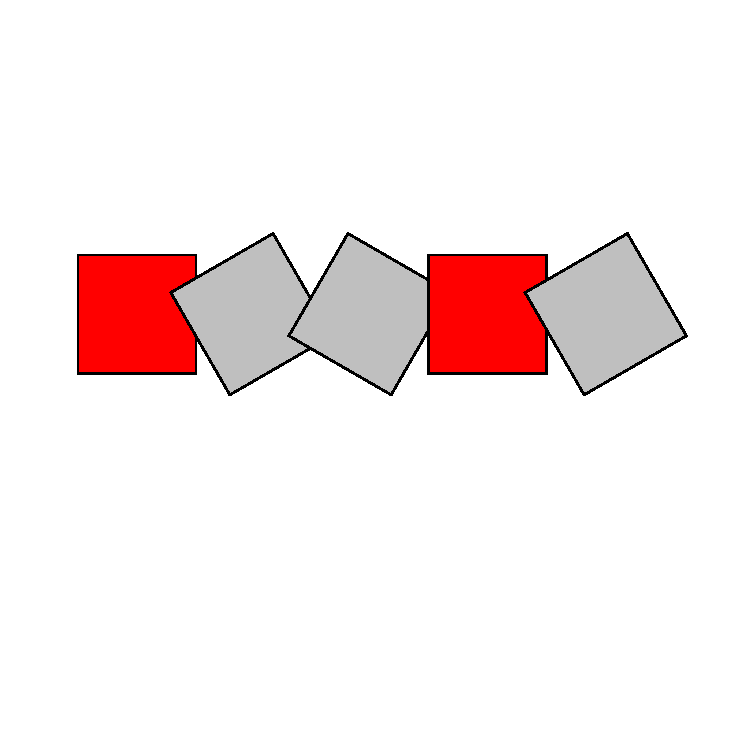
\includegraphics[width=0.5\textwidth]{SquareRotate}
	\end{center}
	\caption{Symmetry of The Square}
    \label{fig:symsquare}
\end{figure}

Actions that preserve the square shape can be combined.
For example, if the action of $90$ degree clockwise rotation preserves the shape, then the action of rotating twice, i.e., $180$ degree clockwise rotation also preserves the shape.

All the actions that can preserve the symmetry form a group $G$.
A group has the following properties.
\begin{enumerate}
\item For any $g_a,g_b$ in $G$, \,$g_a*g_b$\, belongs to $G$. (The operation ``$*$'' is closed).

\item For any \,$g_a,g_b,g_c\in G$, \,$(g_a*g_b)*g_c=g_a*(g_b*g_c)$. \,(Associativity of the operation).

\item There is an element $e\in G$ such that \,$g_a*e=e*g_a=g_a$\, for any \,$g_a\in G$. (Existence of identity element).

\item For any \,$g_a\in G$\, there exists an element $g_h$ such that \,$g_a*g_h=g_h*g_a=e$. \,(Existence of inverses).
\end{enumerate}

For the square example, all the actions preserve the square shape form the group $G$.
$g_1$ is  $90$ degree clockwise rotation, identity element $e$ is the action of no rotation,
$g_2=g_1*g_1$ is the action of rotating $90$ degree clockwise twice.
Since $g_2$ preserves symmetry, $g_2$ is an element of the group $G$, 


From the algebraic perspective, ``Symmetry'' means the value of function is invariant after transformation.
For a function $I(x)$,
the group transformation is define by $\tilde{x}=g_a(x)$.
By symmetry, we mean $I(x)=I(\tilde{x})$.
$I(x)$ is an invariant function of group $G$.


Note that  shapes invariant by actions in $G$  are not unique.
Many shapes are invariant, and their combinations are also invariant, as shown in Figure~\ref{fig:SymmetrySpace}. 
In the algebraic sense,  invariant functions of group $G$ form a space, the invariant space $I^G$.


\begin{figure}[!htbp]
  \begin{center}
    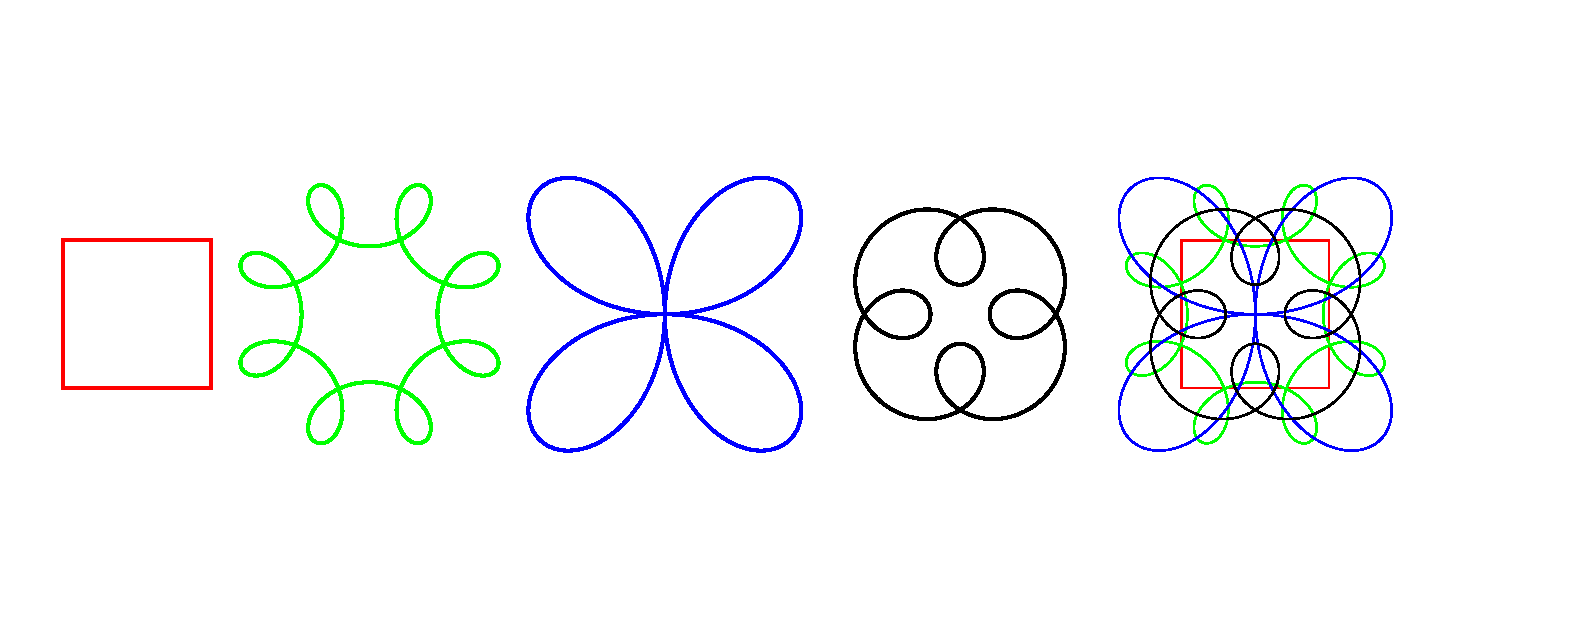
\includegraphics[width=0.7\textwidth]{ShapeCombination}
    \caption{Two invariant Shapes and the invariant combination}
    \label{fig:SymmetrySpace}
\end{center}
\end{figure}

\subsection{Lie Group and Differential Equation}
Physically-based motions are usually described by differential equations, and motion is the solution of the equation.
Same as the square shape, there are also symmetry groups that keep the differential equations invariant.
An important property of such a group  is that its elements can transform the solution of differential equations from one into another\citep{olver1986applications}.
For \cms, this property  can potentially help reduce computational burden: new motions can be achieved through applying  transformation to the dynamic equations of motion primitives.




In mathematical theory, \emph{Lie Group} is continuous group, which is also a manifold.
Since it is a manifold, coordinate system can be assigned to a Lie Group and each elements can be parameterized.
For example, the symmetry rotation group of square is discrete, while symmetry group of circle is continuous.
For the symmetry group of the circle, each element can be parameterize by the the rotation angle.
In the following discussions,  $\ep$ is the parameter of a element $g$ in the group $G$.

Theory of Lie group comes from the study of differential equations.
For the differential equation in Equation~\ref{eq:difforg}.
\begin{equation}
\label{eq:difforg}
\dot{\state}=F(\state)
\end{equation}
Invariant function $I$ can be defined as:
\[
I(t,\state,\dot{\state})=F(\state)-\dot{\state}
\]
Solutions of the differential equation are the kernel of the invariant function $I$ :
 \[
 I(t,\state,\dot{\state})=0
 \]
 
 
The group transformation will act on all the variables of the invariant function.
Therefore $t$, $\state$ and $\dot{\state}$ are all transformed.
\[
(t,\state,\dot{\state}) \mapsto (\tilde{t},\tilde{\state},\dot{\tilde{\state}})
\]
If the group $G$ is symmetrical, then value of the  function $I$ will be invariant.
Therefore  the kernel is transformed into kernel, and the transformed variables are still solutions to the original differential equations. 
\[
I(t,\state,\dot{\state})=I(\tilde{t},\tilde{\state},\dot{\tilde{\state}})=0
\]


Note that the $\dot{\state}$ is not independent which depends on the $t$ and $\state$,
\[
\dot{\tilde{\state}}=\frac{d \tilde{\state} }{d \tilde{t}}
\]
From the geometrical perspective, it is not easy to present  the transformation of $t$.
Instead, we define two actions on the state space and tangent space.
In the state space, we define the  action $g$ that transforms the state. 
\[
g(\state)=\tilde{\state}
\]
In the tangent space, we define the \emph{lift action} $Tg$ 
\[
Tg(\dot{\state})=\dot{\tilde{\state}}
\]

$Tg$ can be worked out by formatting the derivatives in the original coordinate system.
For example, the translation $g_{\ep}$ 
\[
(x,y)\mapsto (x+\ep,y+\ep)
\]
$Tg_{\ep}$ is
\[
(\dot{x},\dot{y}) \mapsto (\dot{x},\dot{y})
\]
$Tg$ is the identity element $e$.


In the general cases, $g$ transforms Equation~\ref{eq:difforg} into Equation~\ref{eq:trdiff}
\begin{equation}
\label{eq:trdiff}
Tg(\dot{\state})=F(g(\state))
\end{equation}
If $g$ is symmetrical, Equation~\ref{eq:difforg} and Equation~\ref{eq:trdiff} are equivalent







 	
For example, 
The scaling action is applied to the state space of the mass spring system of Equation~\ref{eq:stateform}. 
\[
\tilde{\state}=g_{\ep}(\state)=[\ep q, \ep \qd ]
\]
then the lift action is
\[
\tilde{\state}=Tg_{\ep}(\state)=[\ep \qd, \ep \ddot{q}]
\]



by substitution $\state \mapsto \tilde{\state}$, the original system becomes
\[ 
\dot{\tilde{\state}}=
\left[ 
\begin{array}{cc}
0 &1\\
-1 &0 
\end{array}
\right]\tilde{\state}
\]
which is 
\begin{equation}
\label{eq:tranmas} 
\ep \dot{\state}=
\left[ 
\begin{array}{cc}
0 &1\\
-1 &0 
\end{array}
\right]\ep \state
\end{equation}

Equation ~\ref{eq:tranmas} is equivalent to  Equation~\ref{eq:stateform}.
If $\state(t)$ is a solution, so is $\tilde{\state}(t)$.

To verify the group property. define $*$ as:
\[
g_{\ep_1}*g_{\ep_2}(\state)=[\ep_1 \ep_2 q, \ep_1 \ep_2 \qd]
\]

The inverse is:
\[
g_{\ep}^{-1}=g_{\frac{1}{\ep}} \;\ep \in R^+
\]

\begin{mydef}
For a group $G$, the invariant function of state $I(\state)$ is called a \emph{local motion invariant} of $G$. 
\end{mydef}

Invariant functions $I(\state)$ has important  meaning in dynamics. 
According  to \textbf{Noether's Theorem}, each $I(\state)$ corresponds to a conservative law. 


\section{Lie Group and Controlled Lagrange}
\label{sec:liecontrol}
It is not enough for animals  only to  explore symmetry groups of natural dynamics for motion adaptation.
For a dynamic system, the symmetry group is quite restricted.  
Working out the symmetry group might be a non-trivial task.
In real-life, animals usually exert control effort during motion adaptations.

\moit\ theory proposes the idea that control effort can make a non symmetrical group become symmetrical, and introduce the \emph{Controlled Lagrange} technique.
Based on biological research\citep{flash2007affine}, some simple groups are selected the symmetry group for motor control.
When such group is applied to the dynamic system, control efforts are applied to ensure the symmetry.


Usually a dynamic system is represented as by Euler-Lagrange Equation~\ref{eq:uncontrolled_euler_lagrange}\citep{Goldstein2002}.
\begin{equation}
\frac{d}{dt} \frac{\partial L}{\partial \qd} - \frac{\partial L}{\partial q} = 0
\label{eq:uncontrolled_euler_lagrange}
\end{equation}

where $L=K-V$, $L$ is the Lagrange, $K$ is the kinetic energy, $V$ is the potential energy, $q$ is the generalized coordinates, and $\qd$ is the generalized velocity.

By applying the group transformation $g$, both the generalized coordinates and generalized velocity will be changed:
\[
g(\state)=\tilde{\state}=[\tilde{q}, \dot{\tilde{q}}]
\]
The Euler-Lagrange equation for the transformed dynamic system is described by Equation~\ref{eq:liegroup_euler_lagrange}.
If control is applied, the Euler-Lagrange equation of the controlled dynamics is described by Equation~\ref{eq:controlled_euler_lagrange}. 
If symmetry is persevered, the two equation should be equivalent.
Then symmetry control input $\ulocal$ can be calculated by comparing the two equations.
\begin{align}
\frac{d}{dt} \frac{\partial L}{\partial \dot{\tilde{q}}} - \frac{\partial L}{\partial \tilde{q} }&=0,\label{eq:liegroup_euler_lagrange}\\
\frac{d}{dt} \frac{\partial L}{\partial \qd} - \frac{\partial L}{\partial q}&=\ulocal. \label{eq:controlled_euler_lagrange}
\end{align}

When the two equations are equivalent, their Lagrange $L$, Kinetic Energy $K$ and potential energy $V$ should be the same or of the same scale factor.
Thus in theory, two strategies exist and will result in two different $\ulocal$:
we can calibrate the kinetic by scaling and apply control effort to compensate the difference in potential energy, or calibrate potential energy and compensate the kinetic energy.
\moit\ adopts the potential shaping strategy, for it is computational efficient and suitable for muscle like biological actuators.
As a special case, potential energy shaping for homogeneous group or affine group promises a close form formulation.
Several groups and their potential shaping control effort are as below:



\subsection*{ Offset Action}
Offset actions  modify the generalized coordinate $q$ by a constant, while speed and time remain unchanged.
Given the offset parameter $\ep$, the mapping will be in the following form:
\[
(t,q,\qd) \mapsto (t,q+\ep,\qd)
\]

The corresponding state transformation and lift action are
\begin{align}
\goff(\state) &= [q+\ep,\qd] \\
T\goff(\dot{\state})&=\dot{\state}=[\qd,\qdd]
\end{align}


On the phase plot,  the configuration $q$ is usually represented by the horizontal axis, and the generalized speed $\dot{q}$ is represented by the vertical axis.
From the geometrical perspective, offset actions will move the phase portrait horizontally as shown in Figure~\ref{fig:goff}.

\begin{figure}[!htbp]
  \begin{center}
      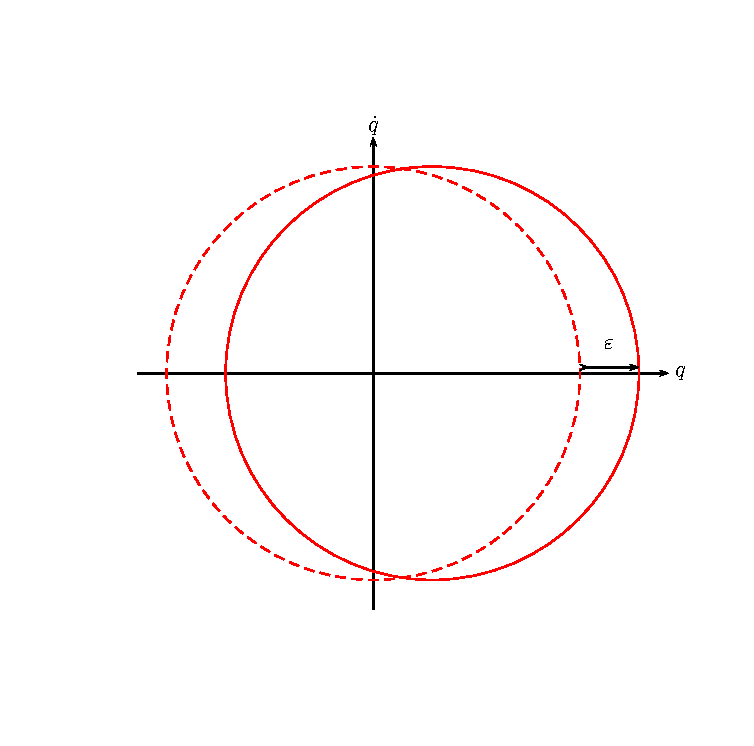
\includegraphics[width=0.5\textwidth]{OffsetAction}
    \caption{Offset Action}
    \label{fig:goff}
\end{center}
\end{figure}

Substituting the transformed $q$ and $\qd$ into Equation~\ref{eq:liegroup_euler_lagrange} and Equation~\ref{eq:controlled_euler_lagrange},
the control input  can be worked out in the following closed form formula:
\begin{equation}
\ulocal(q) = \frac{\partial}{\partial q} \left(V(q)-V(\tilde{q}) \right).
\end{equation}

Taking the mass spring system of Equation~\ref{eq:mass-spring} as an example, the transformed equation  and control equation are as follows.
\begin{align}
\ddot{\tilde{q}}+\tilde{q}-\ep&=0 \nonumber \\
\ddot{q}+q&=\ulocal \nonumber
\end{align}
By comparing the two equations, we work out that:
\[
\ulocal(q)=\ep
\]




\subsection*{Time Scaling}

%g_st(q,dot{q})=(q,st*dot{q})
Time scaling actions divide the time variable by a factor $\ep$.
The generalized coordinates are kept unchanged, and the generalized speed will be multiplied by $\ep$.
For the action of parameter $\ep$, the action mapping is: 


\[
(t,q,\qd) \mapsto (\frac{t}{\ep},q,\ep \qd)
\]

The corresponding state transformation and lift action are
\begin{align}
\gts(\state)&=[q,\ep \qd] \nonumber \\
T\gts(\dot{\state})&=[\ep \qd,\ep^2 \ddot{q}]\nonumber
\end{align}

From a geometrical perspective, time scaling will stretch the phase portrait vertically, as shown in Figure~\ref{fig:gts}.
\begin{figure}[!htbp]
  \begin{center}
    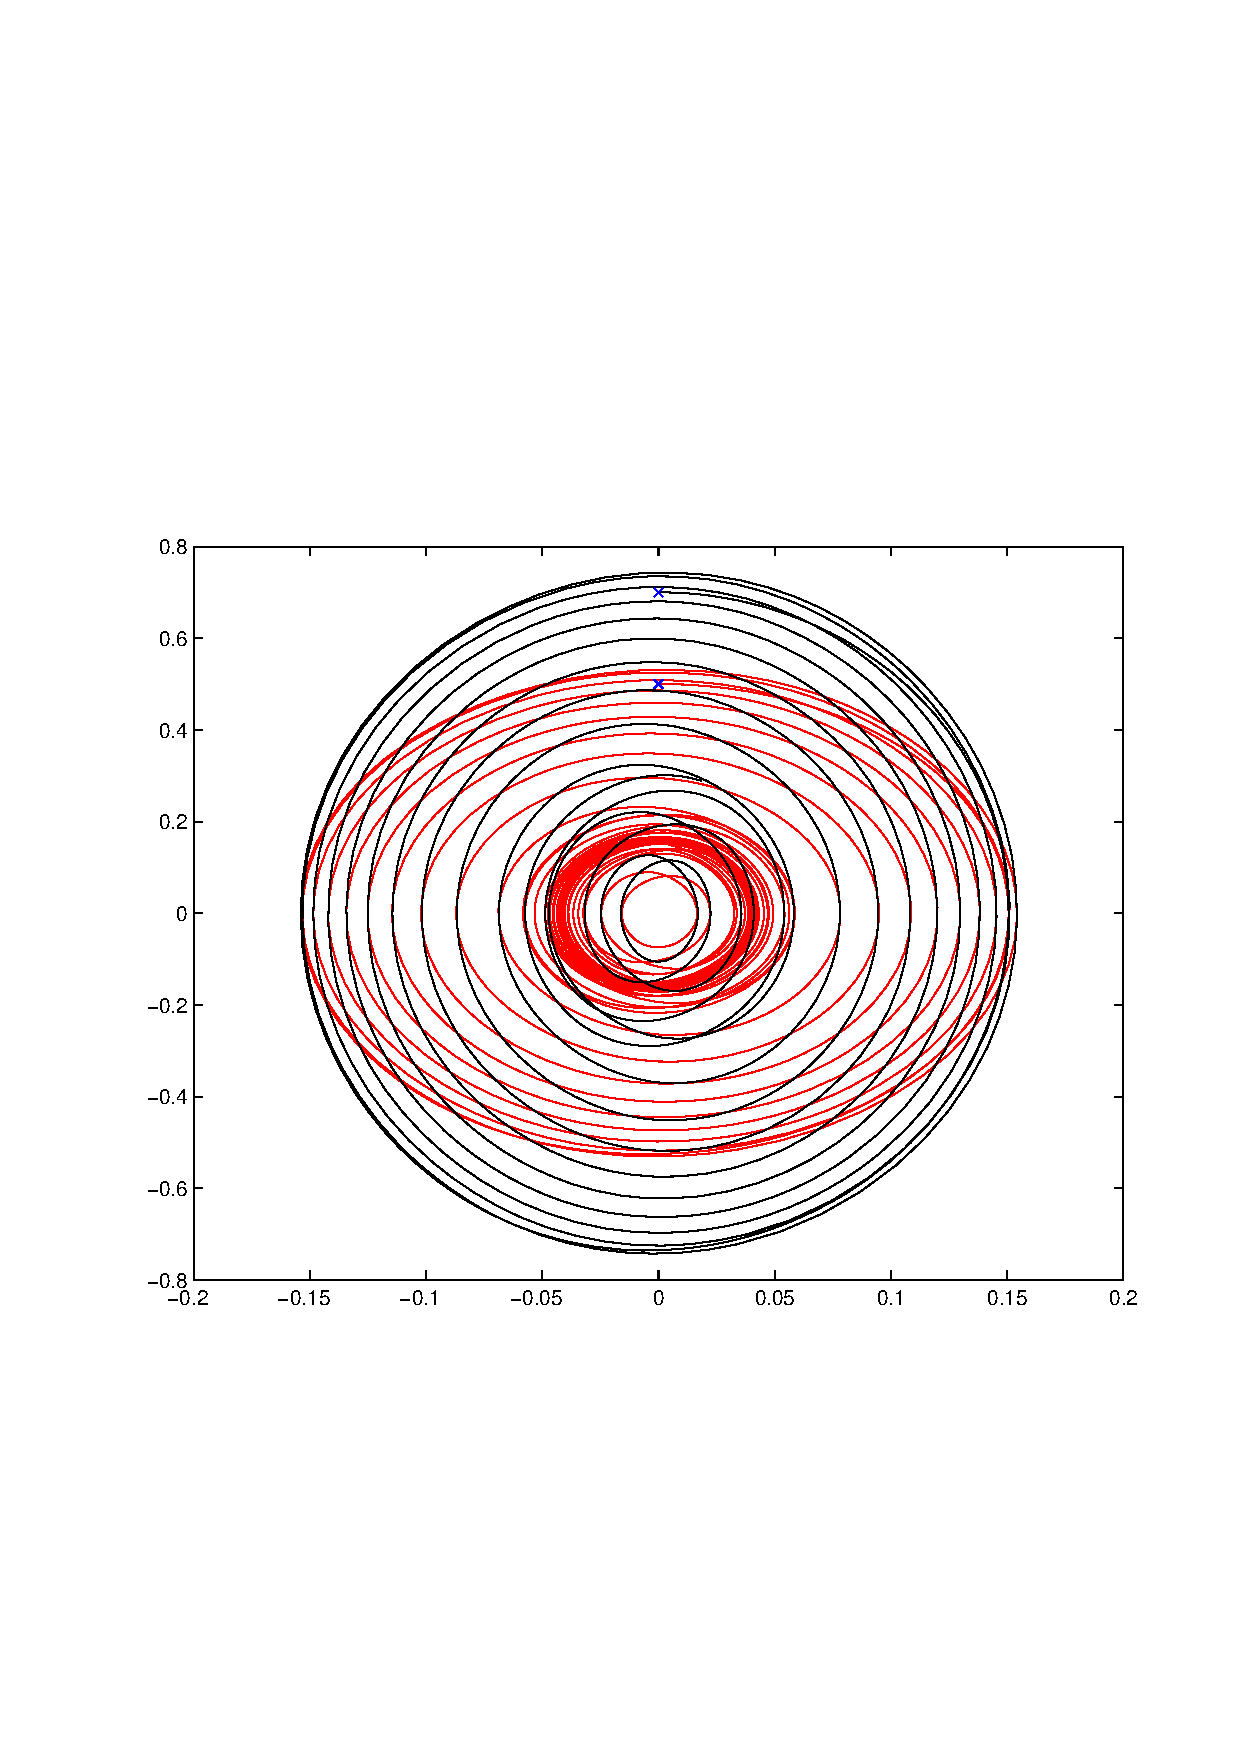
\includegraphics[width=0.5\textwidth]{TimeScaling}
	 \caption{Time Scaling Action}
    \label{fig:gts}
\end{center}
\end{figure}

The control input can be worked out in the same manner as offset actions.
There is also a closed form formula for control input.
\begin{equation}
\ulocal(q) = (1-\ep^2) \frac{\partial V(q)}{\partial q}.
\end{equation}

Again, taking the mass spring system of Equation \ref{eq:mass-spring} as an example, the transformed and controlled equations are

\begin{align}
\frac{\ddot{\tilde{q}}}{\ep^2}+\tilde{q}&=0 \nonumber \\
\ddot{q}+q&=\ulocal \nonumber
\end{align}
The local control input is:
\[
\ulocal=(1-\ep^2)q
\]




\subsection*{Energy Scaling}
For the  dynamic system of the conservative field,
the energy is preserved in motion and different motions are characterized by their energy.
For such a system, motion can be adapted by modifying the energy of the dynamic system.

Energy Scaling action is introduced to adapt motions.
The scaling transformation has the following property:
\[
E(\tilde{\state})=\ep^2 E(\state)
\]
where $E$ is the energy, defined as $E(\state)=K+V$,  $K$ is the kinetic energy, and $V$ is the potential energy.

Further suppose that both the potential and kinetic energy are transformed uniformly.
\begin{align}
K(\tilde{\state})=\ep^2 K(\state) \nonumber\\
V(\tilde{\state})=\ep^2 V(\state) \nonumber
\end{align}
When mass inertia matrix is constant,  the energy scaling transformation is linear as follows:
\[
(t,q,\qd ) \mapsto ( \frac{f(\ep)}{\ep}t ,f(\ep)q,\ep\qd)
\]
$f(\ep)$ is a function of $\ep$, which is determined by the conservative field.
Geometrically, an energy scaling action enlarges the phase portrait,as shown in Figure~\ref{fig:gen}.
\begin{figure}[!htbp]
  \begin{center}
      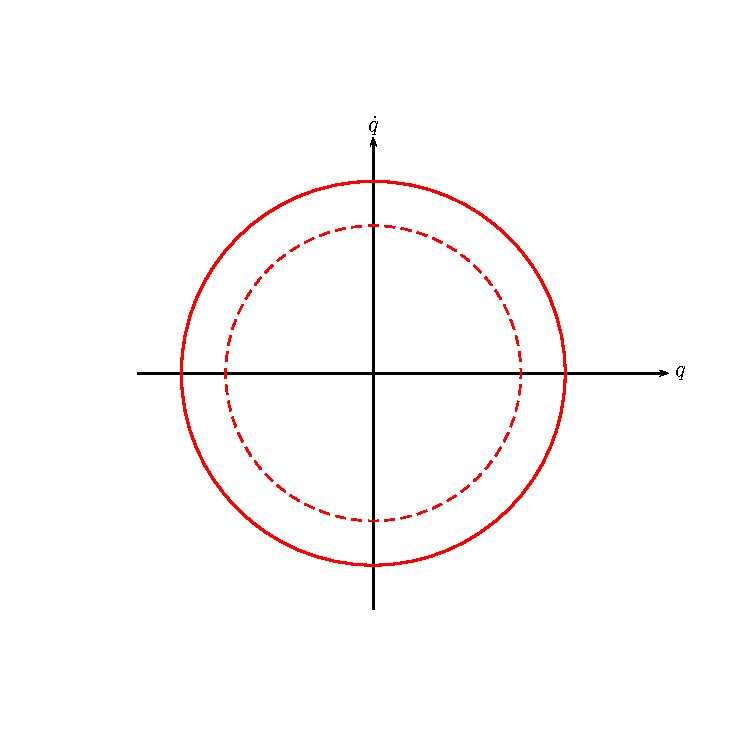
\includegraphics[width=0.5\textwidth]{EnergyScaling}
    \caption{Energy Scaling Action}
    \label{fig:gen}
\end{center}
\end{figure}

The corresponding  state transformation and lift action are:
\begin{align}
\gen(\state)&=(f(\ep) q,\ep \dot{q}) \nonumber\\
T\gen(\dot{\state})&=(\ep \dot{q},\frac{\ep^2}{f(\ep)}\qdd)
\end{align}

$\ulocal$ can by worked out in the same manner as the above actions.
Rather than write down the closed form formula, the thesis prefers an alternative process.
Energy Scaling can be seen as a combined action of two actions: scaling the generalized coordinates and scaling the time variable.
Separate formula can be developed for two actions independently.
This principle generates modular code structure.




The mass spring system of Equation\ref{eq:mass-spring} is selected again as an example.
 For the mass spring system, Energy is defined as~$E=\frac{1}{2}(q^2+\qd^2)$.
 If the energy is scaled up by $\ep^2$,  the potential energy is scaled up by $\ep^2$.
 Because $V= \frac{1}{2}q^2$, and $\ep^2 V=\frac{1}{2}(f(\ep)q)^2$, thus $f(\ep)=\ep$.
 
 
The control input can be worked out in the same manner as the above actions.
However, when object moved in the conservative field, energy scaling is a symmetry group of the original dynamic system, thus no control effort is needed.
\[
\ulocal=0
\]



\subsection*{Time Offset}

Time offset actions modify the time  variable $t$ by the parameter~$\ep$.
The map is as follows
\[
(t,q,\qd) \mapsto (t+\ep,q,\qd)
\]


For a system oscillating with limit cycle, time offset action will modify the phase, as shown in Figure~\ref{fig:gtoff}.
\begin{figure}
  \begin{center}
      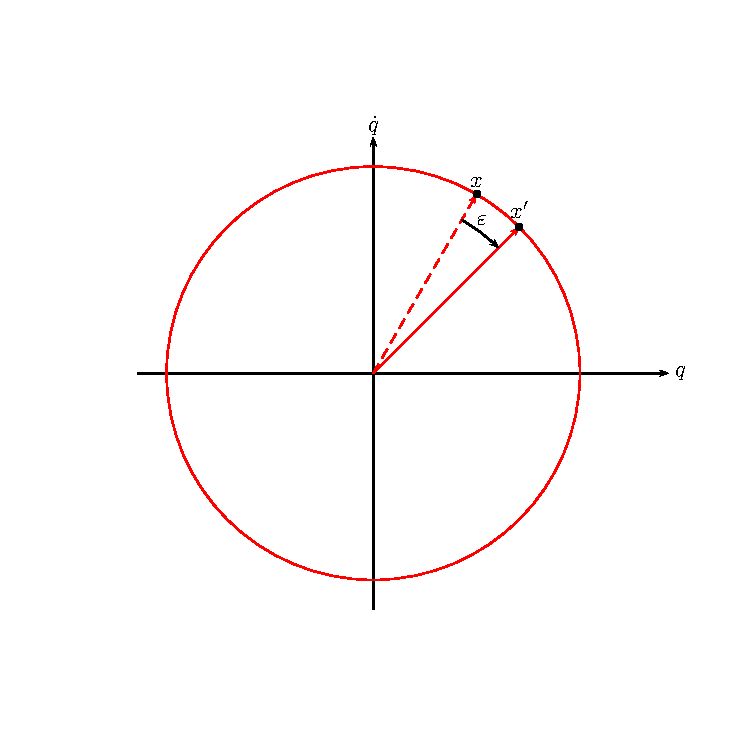
\includegraphics[width=0.5\textwidth]{TimeOffset}
    \caption{Offset Action}
    \label{fig:gtoff}
\end{center}
\end{figure}

For a dynamic system, time offset is symmetrical for all dynamic system.
At the first look, no control effort is needed.
In practise, time offset is achieved by applying time scaling twice, after applying time scaling $\ep$ for sometime, and then apply the inverse action(time scaling of $\frac{1}{\ep}$).


\subsection{Action Selection}
There are many actions available for motion adaptation.
In certain situations, there are many different ways to satisfy the motion constraints, causing the problem which action should be applied.
Different groups will result in different motion styles.
This idea is supported by lots of examples in Chapter~\ref{chap:walk}.
In practise, this is left for the animator to decide.
Usually, the symmetry of natural dynamic is preferred, for such actions are energy efficient.







\section{Example: Symmetry of the Bouncing Ball System}
\label{sec:symball}
Symmetry is a common property among many dynamic systems, even for the hybrid systems like the bouncing ball system of Equation~\ref{eq:bbeq}.
It is shown in this section that by utilizing the symmetry group, complex motions can be predicted in an computationally efficient way.

The bouncing ball system of~\ref{eq:bbeq} has a energy scaling symmetry.

The energy function of the bouncing ball system is  
\[
E=\mathrm{g}q+\frac{1}{2}m\qd^2
\]
If the energy is scaled up by $\ep^2$,  potential energy is scaled up by $\ep^2$.
 Because $V= \frac{1}{2}\mathrm{g}q$, and $\ep^2 V=\frac{1}{2}f(\ep)q$, thus:
\[
f(\ep)=\ep^2
\]
the energy scaling transformation is
\[
\gen(\state)=[\ep^2 q, \ep \qd]
\]

For the bouncing ball system, the energy of a system can be characterized by the initial dropping height.

Given the motion of a ball dropped at $5$ as shown in Figure~\ref{fig:bouncing5}, we set $\ep=\sqrt{2}$ and obtained the motion dropped from $10$ through the transformation as shown in Figure~\ref{fig:bouncing10}.
Figure  motion dropped from $10$ is shown in Figure~\ref{fig:bouncing10sim}.
\begin{figure}[!htbp]
  \begin{center}
      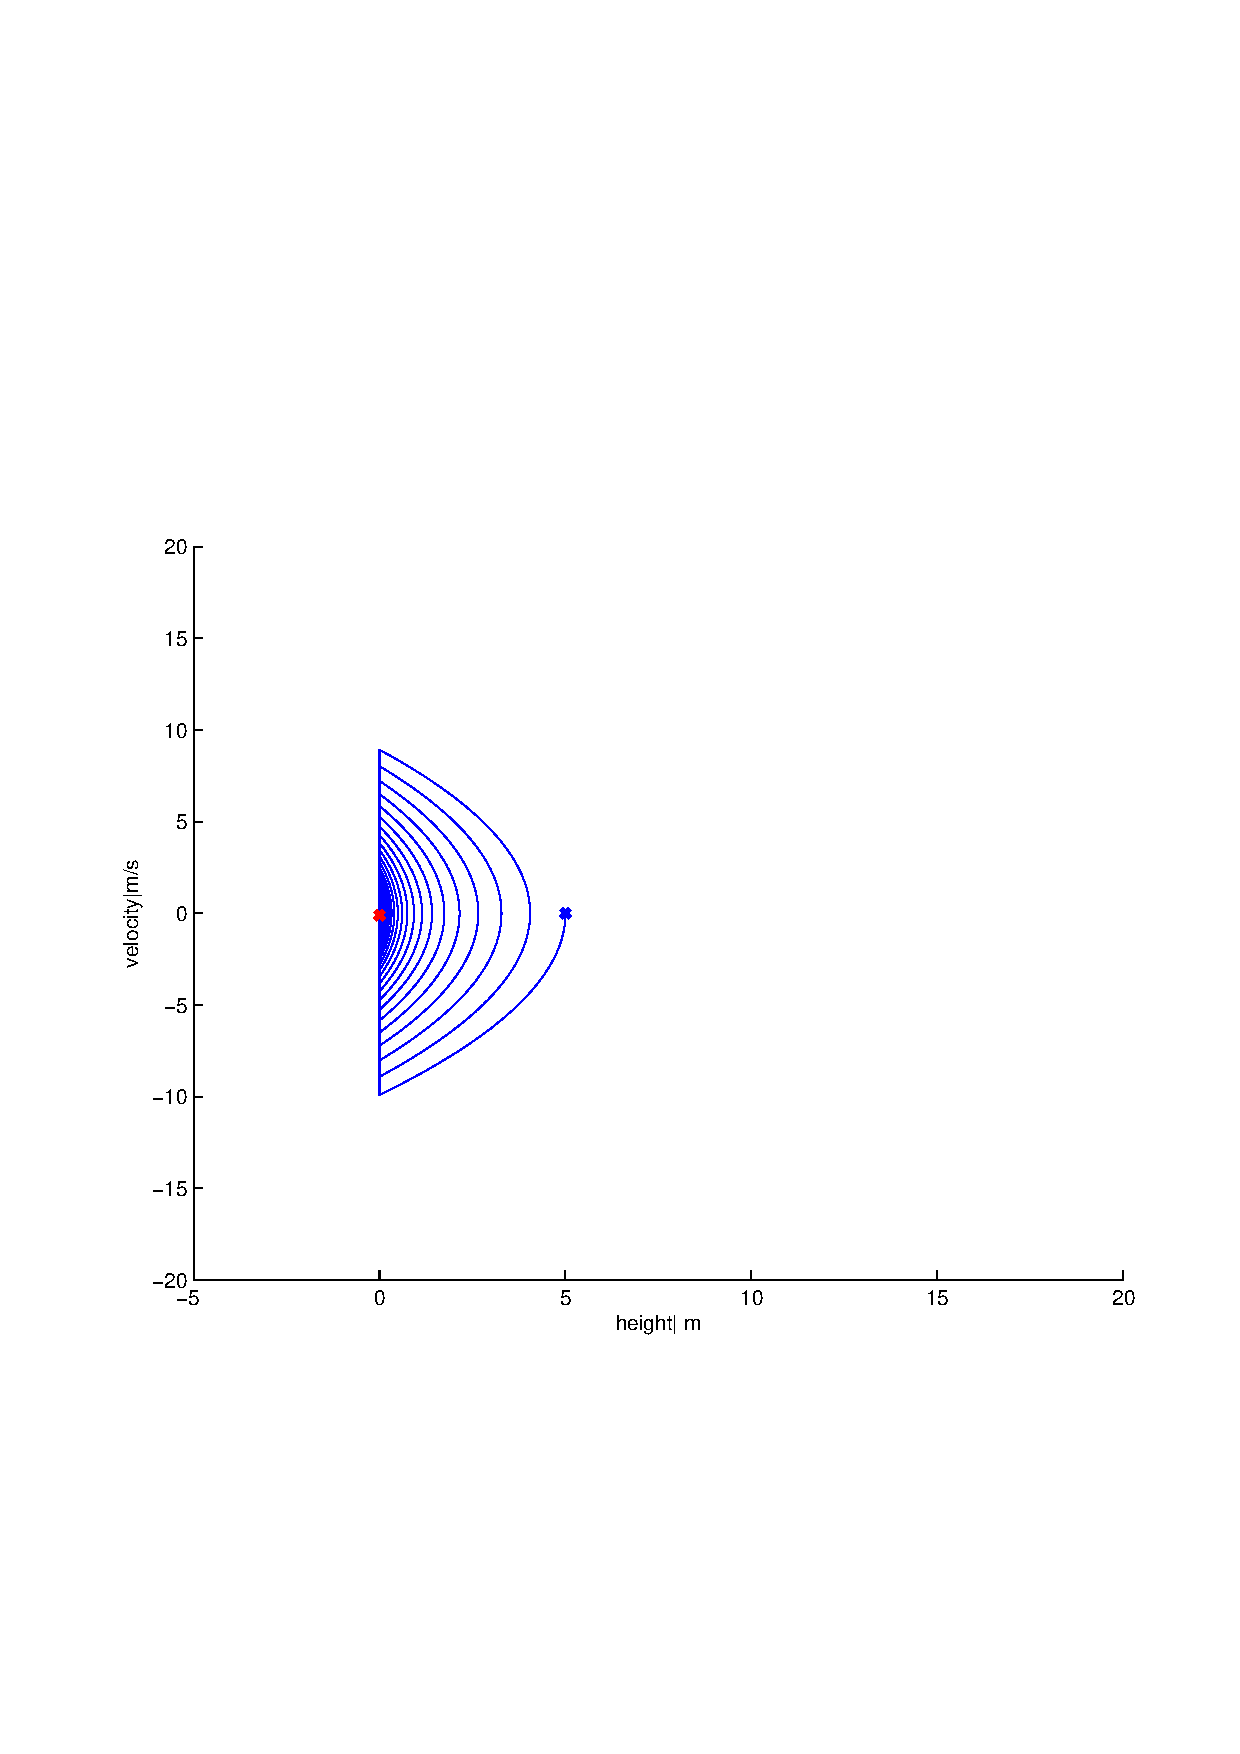
\includegraphics[width=0.5\textwidth]{BouncingBallPhasePlotuncontrolledDropAt5}
    \caption{Drop at 5}
    \label{fig:bouncing5}
\end{center}
\end{figure}


\begin{figure}[!htbp]
  \begin{center}
      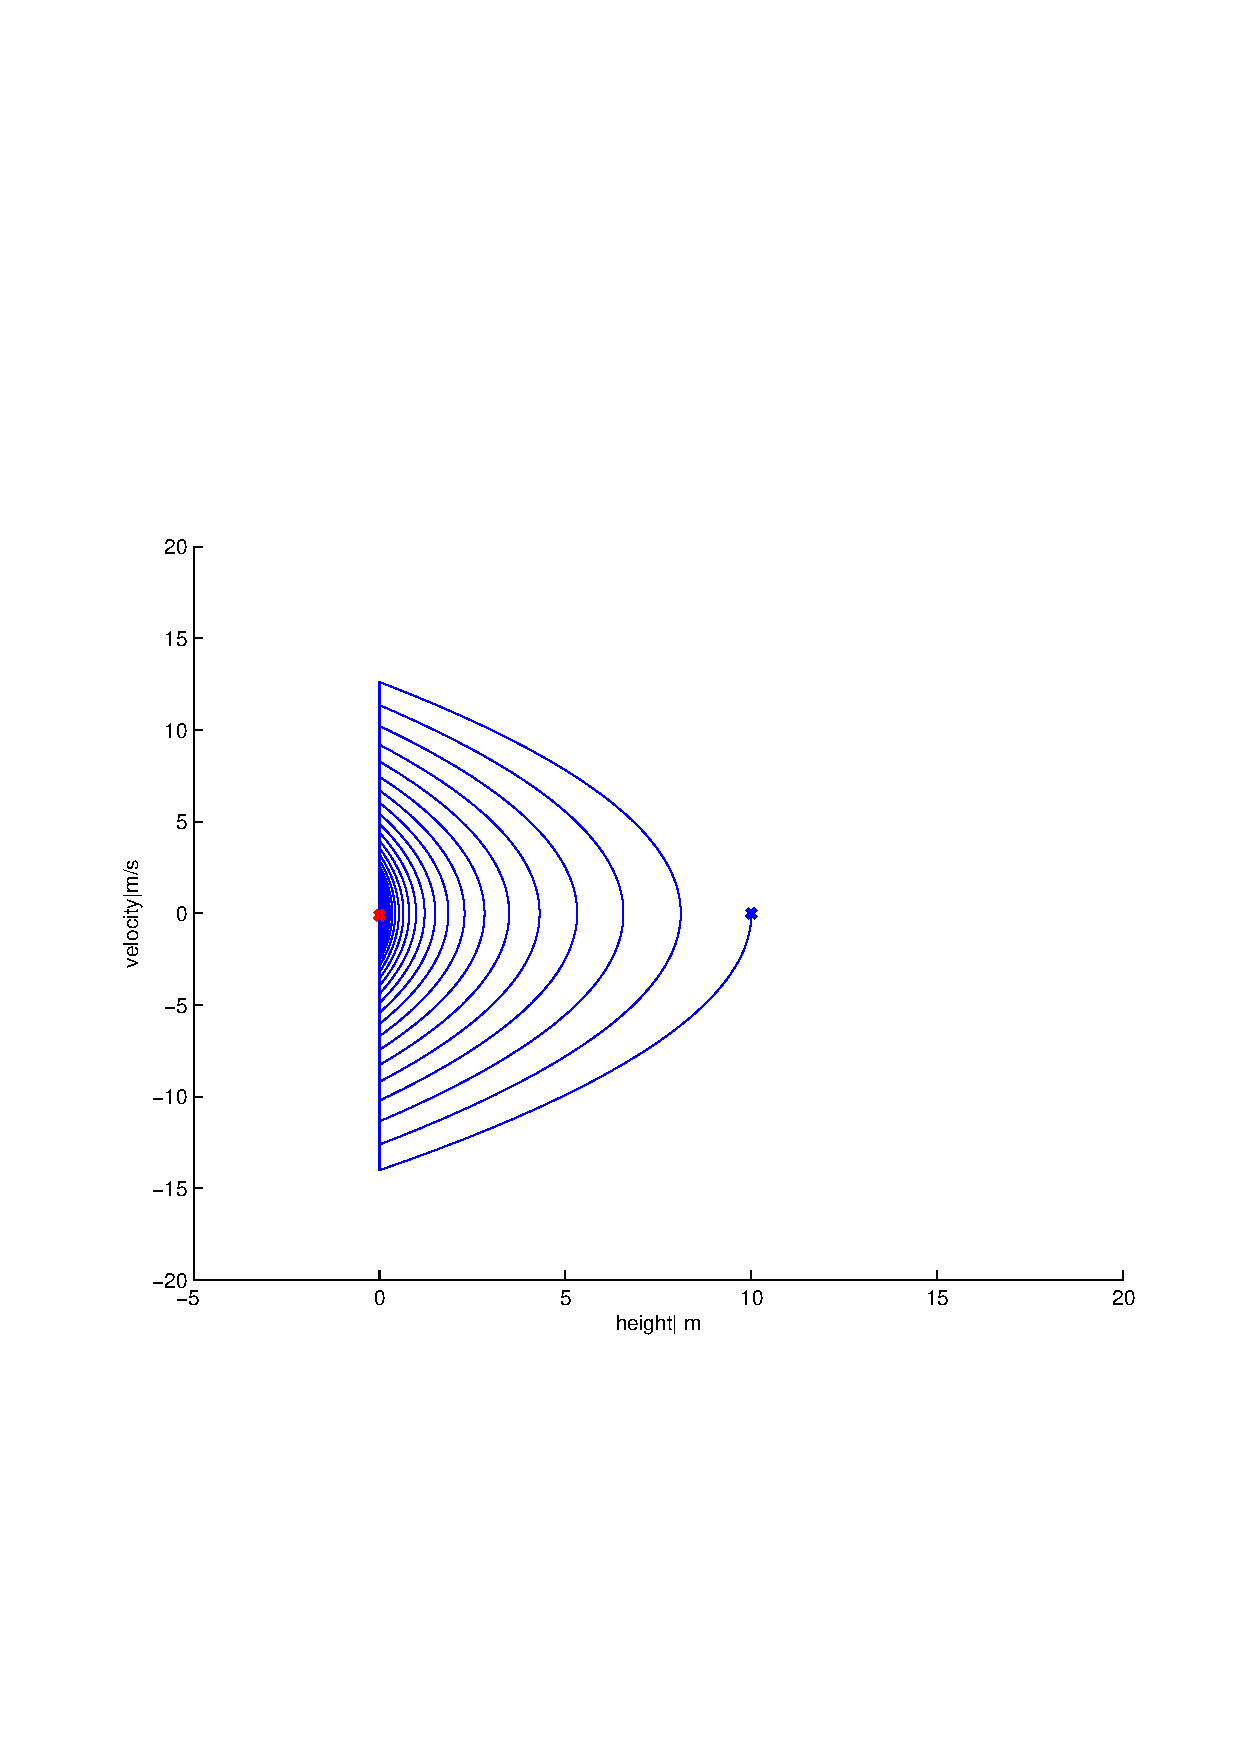
\includegraphics[width=0.5\textwidth]{BouncingBallPhasePlotuncontrolledDropAt10}
    \caption{Drop at 10 by transformation}
    \label{fig:bouncing10}
\end{center}
\end{figure}

\begin{figure}[!htbp]
  \begin{center}
      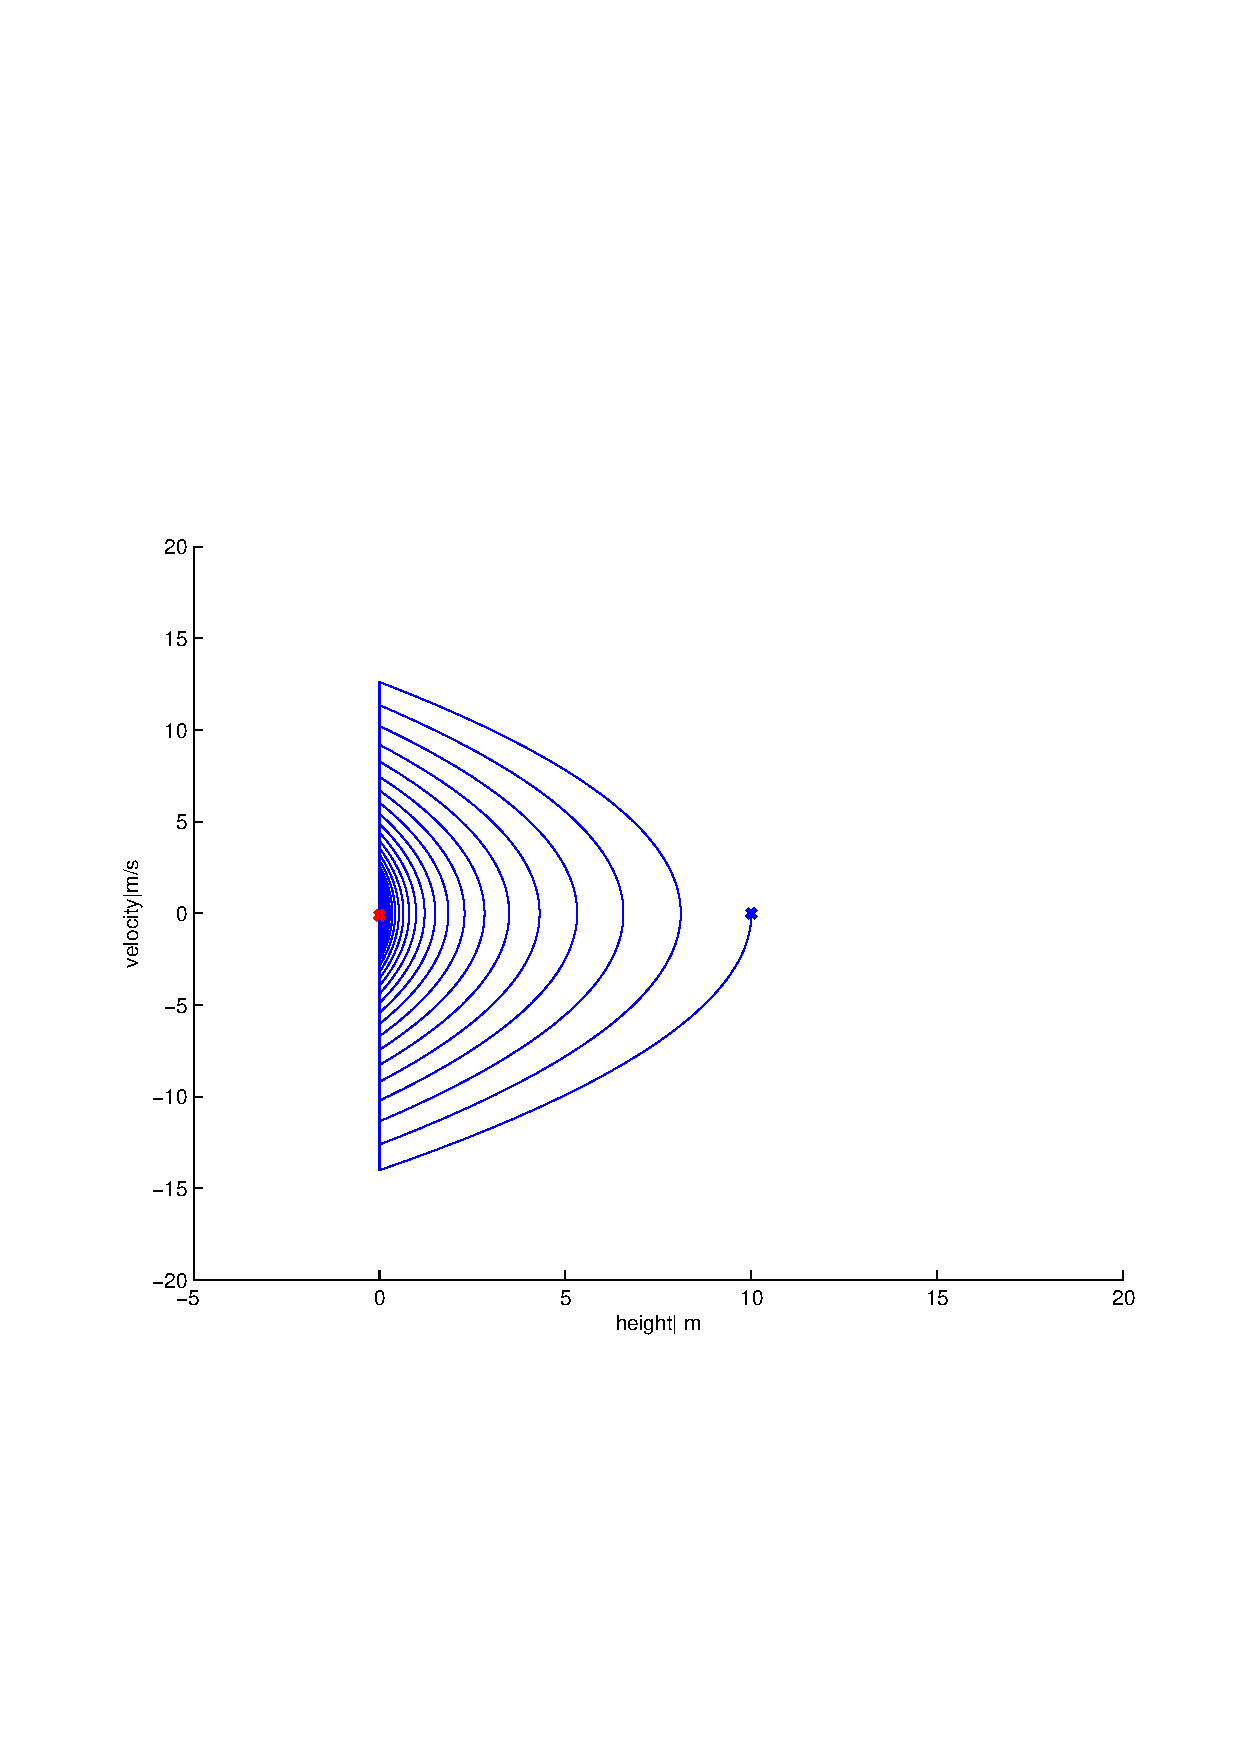
\includegraphics[width=0.5\textwidth]{BouncingBallPhasePlotuncontrolledDropAt10}
    \caption{The simulation result of dropped from 10}
    \label{fig:bouncing10sim}
\end{center}
\end{figure}



